% Setup
\documentclass[a4 paper, 12pt]{article}

% Title
\title{MEDIUM FIDELITY}

% Margins
\usepackage{geometry}
\geometry{margin=2cm}

% Images
\usepackage{graphicx}
\usepackage{float}
\usepackage[export]{adjustbox}
\setlength{\intextsep}{5pt plus 2pt minus 2pt}
\setlength\belowcaptionskip{0ex}
\usepackage[font=footnotesize,skip=2pt]{caption}

% Paragraph
\setlength{\parindent}{2em}
\setlength{\parskip}{1em}

% Text Formatting
\usepackage[utf8]{inputenc}
\usepackage[english]{babel}

% List spacing
\usepackage{enumitem}
\setlist{noitemsep, topsep=0pt}
\setlist[enumerate]{parsep=2pt} 

% Text Color
\usepackage{xcolor}

% Hyperlinks
\usepackage{hyperref}
\hypersetup{
    colorlinks=true,
    linkcolor=black,
    filecolor=black,      
    urlcolor=blue,
}

% Appendix
\usepackage{appendix}

% Include pdf
\usepackage{standalone}
\usepackage{pdfpages}

% Borders
\usepackage{mdframed}

% Symbols
\usepackage{amssymb}

\usepackage{multicol}
%%%%%%%%%%%%%%%%%%%%%%%%%%%%%%%%%%%%%%%%%%
\begin{document}

% 3.2 MEDIUM FIDELITY PROTOTYPE
\section{Iteration 2 - Medium Fidelity Prototype}
The medium fidelity prototype is the first digital version of the application. It follows the research and initial conceptual design of the low fidelity prototype, while revising these concepts using the analysis of the first round of evaluations. The main sections of misunderstanding are from restaurant to comparison list, and comparison list to restaurant. To better understand the users and the usability of the app, this section additionally includes personas, scenarios and UX Goals. 

% The prototype can be viewed \href{https://www.figma.com/proto/0WYtAGvFm8aOhxSIDqGJ4R/Medium-Fidelity?node-id=4%3A3&scaling=scale-down}{here}.

% 3.2.1 REVISED REQUIREMENTS/CONCEPTUAL DESIGN
\subsection{Revised Requirements/Conception Design}
From the low fidelity evaluations the initial requirements and conceptual designs will be revised accordingly. This includes more detail to the design principles and system requirements. Additionally, personas and interaction scenarios for each will be introduced to empathise with the user, and UX goals identified to assist with measuring usability.

    \subsubsection{System Concept Statement}
    The problem statement and high-level description of the outlined in the low fidelity prototype are still accurate for the next iteration, as well as the definition of mobile paradigm and instructing mode. However, whilst most of the metaphors were accurately chosen, there were several that either didn't align with the user's mental models or the defined design principles. The following updated metaphors will be applied to this next iteration, as per the evaluation analysis of the low fidelity prototype.
        \begin{itemize}
            \item bookmark $\dashrightarrow$ scales \\
            \textit{Didn't match the mental model of users for 'Editable and shareable list' feature}
            \item map with location marker $\dashrightarrow$ compass \\
            \textit{Wasn't consistent with industry standards for 'EXPLORING' action, violating design principle 'Be Familiar'}            
            \item coupon $\dashrightarrow$ offer \\
            \textit{Wasn't consistent with industry standards for 'DEALS' representation, violating design principle 'Be Familiar'} 
        \end{itemize}


    \subsubsection{Design Principles}
    From the evaluation analysis of the low fidelity prototype, it was evident that only two of the design principles identified in the first conceptual design were followed satisfactory.   
    \begin{itemize}
        \item Open to change - All users stated that their attitude towards the app (during the TAM evaluation) would improve if their suggestions from the co-design were implemented, all of which will be in this following iteration.  
        \item Manageable steps - There was no issue with the flow of the application and users appreciated the use of tabs [45].
    \end{itemize}
    
    The remaining design principles were not implemented well enough causing issues for the users which particularly affected their perceived ease of use and attitude towards the application.
        \begin{itemize}
            \item Simplify decision process - All users encountered at least one issue, either during the gulf of execution or evaluation, that prevented them from moving forwards without assistance. During this next iteration, these issues will be resolved and more attention will be made to preventing these serious errors by making all action buttons more visible and accessible.
            \item Give clear direction and guidance - Most users were unable or unsure of how to move from finding a restaurant to going there. In this next iteration there needs to be more focus by providing large actionable buttons.
            \item Be familiar - One of biggest confusions was with the word and icon choice for list. In this iteration this will be changed to scales metaphor and 'compare'. 
            \item Encourage collaboration - Users weren't aware that the recommendation system was based on word-of-mouth only, and so in this iteration the text 'friends' will be added to be clear.
            \item Maximise customisation opportunities - Users weren't aware that their filtering of preferences also extended to the menu. The same filtering element as the interactive map will be applied on the map page to ensure users are aware of the extent of their customisation abilities.
        \end{itemize}

    Additionally, two new design principles were identified following the low fidelity evaluations and will be introduced in this iteration to contribute to these guidelines. 
        \begin{itemize}
            \item Fluid navigation - Users weren't able to move smoothly back and forth between pages which added steps to their process. In this iteration, users should be able to get to a stage of can't continue and will be resolved by providing more actions on pages.
            \item Immediate access to actions - Once reaching the comparison page, users wanted access to more action options then just directions. In this iteration they will be given additional options readily available on the same page.
        \end{itemize}

    In order to satisfy these principles and those previously stated, the below will be taken into consideration for the prototype. Many of these design elements respect existing platform guidelines to ensure both visual and functional consistency across the application to reduce confusion for the users [5]. The well documented industry standards outlined by material design will be followed. These standards are not only thoroughly researched to ensure the optimal user experience, but their popularity creates a sense of familiarity for users which greatly reduces cognitive load (especially in terms of memory, learning, and pattern and recognition) [5, 30, 38]. 
        \begin{itemize}
            \item Colour
                \begin{itemize}
                    \item Consistent colour throughout: The primary colour, used for a majority of the application, is 'medium violet red'. This colour was selected as pink is calming, joyful and encourages creativity [7], which aligns with the aim of wanting to users to enjoy the experience of choosing where to dine out.
                    \item Follow recognizable colour schemes: Variants of the primary colour are used in contrast to distinguish different elements [60]. They were chosen using the material design palette generator [58]. The light variant is 'lavender blush' and is used to fill buttons when they are selected. This follows a monochromatic scheme which produces a soothing effect and is easy on the eyes [1, 2]. By using specific colours this also assists with reducing cognitive overload using the Gestalt principle of similarity [40, 65].   
                    \begin{figure} [H]
                        \centering
                        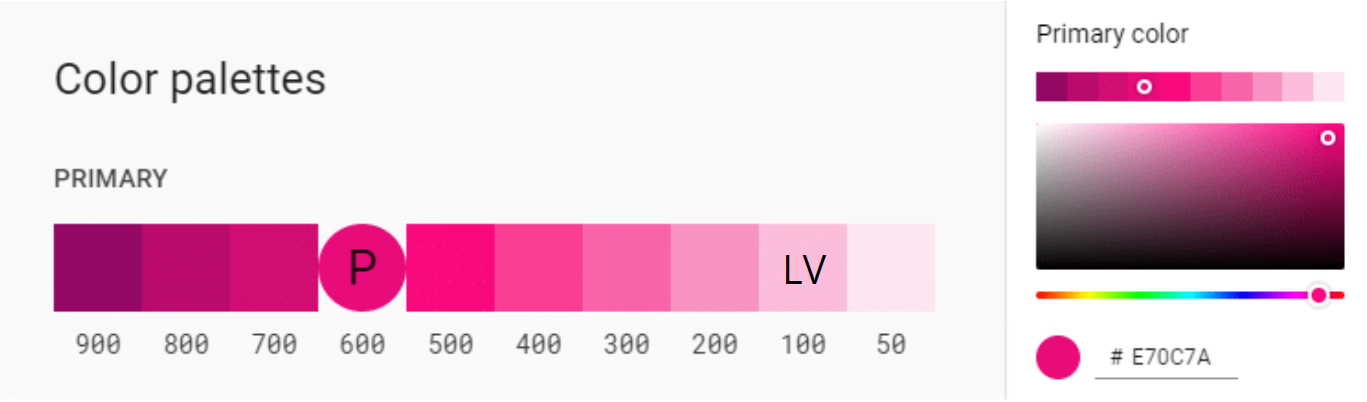
\includegraphics[width=0.8\textwidth, frame]
                            {./Med_Fidelity/Med_Report/images/colour_med.PNG}
                            %{./images/colour_med.PNG}
                        \caption{Colour Palette - Medium Violet Red [58]}
                    \end{figure}
                \end{itemize}

            \item Typography
                \begin{itemize}
                    \item Use popular font: The only font used throughout the app is 'roboto'. It is the default font for Android and many Google services [55]. The colour of the font is either the primary, white or grey depending on the background.
                    \begin{figure} [H]
                        \centering
                        
\includegraphics[width=0.8\textwidth, frame]
                            {./Med_Fidelity/Med_Report/images/font.PNG}
                            %{./images/font.PNG}
                        \caption{Font - Roboto}
                    \end{figure}                    
                \end{itemize}

            \item Iconography
                \begin{itemize}
                    \item Use industry standards metaphors: The appearance of the icons is in-line with material design where possible [59]. Some of these icons take advantage of closure in Gestalt's theory (users complete borders themselves) [40, 51]. The only icon that had to be sourced elsewhere was the scales for the compare feature.  
                    \begin{figure} [H]
                        \centering
                        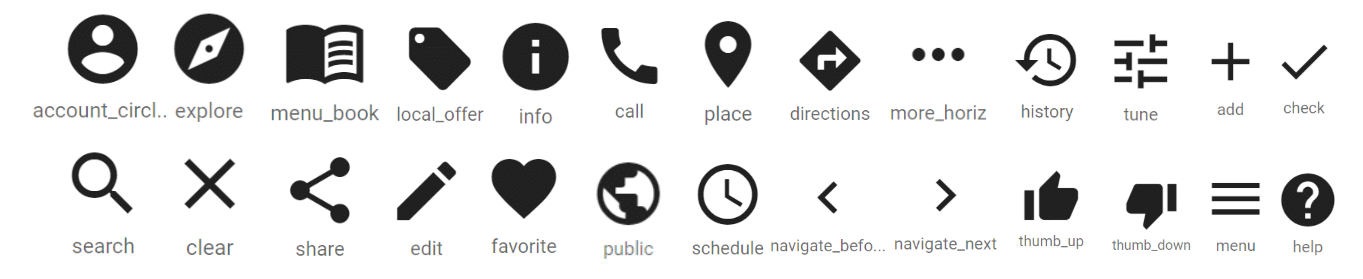
\includegraphics[width=0.9\textwidth, frame]
                            {./Med_Fidelity/Med_Report/images/material_icons.PNG}    
                            %{./images/material_icons.PNG}
                        \caption{Icons - Material Design [59]}
                    \end{figure}   
                \end{itemize}           

            \item States
            \begin{itemize}
                \item Hierarchical visuals (colour, text) - Titles and buttons should be large and primary coloured, to contrast against other elements to allow quick access [3].
                \item Highlight active interfaces - Ensures tabs are coloured when selected to make it clear to users the current page they are on.
            \end{itemize}

            \item Navigation
            \begin{itemize}                
                \item Bottom navigation bar - Provides access to 3-5 top-level destinations. This allows quick movement between screens [4]
                \item Navigation tabs - Used within the restaurant hierarchy to replicate the bottom bar to enable later navigation but for peer related content [4]. Also supports users mental models of tabs [45].
                \item Elements are consistent and locked - Follows the Gestalt principle of continuity [40, 51].
                \item Access to desired buttons - Offer clear affordances, less movement between pages [36].
                \item Large buttons lose to action - Reduced errors and wasted time as per Fitts law [40, 53].
            \end{itemize}
                
            \item Communication 
            \begin{itemize}
                \item Icons accompanied by small text - Although selected icons should be popular metaphors, added text helps to reduce the cognitive load and assist first-time users [4].
                \item Avoid jargon - Everyone should be able to understand any text used throughout the application. For example LIST was not clear and has been amended to COMPARE [5].
                \item Limit number of options - Keep all tabs, dropdowns and menus to under 5 visible options so as not to overwhelm the user as per Hicks Law [40, 54].
            \end{itemize}
            
            \item Space 
                \begin{itemize}
                    \item Dropdown/hidden menus - Follow the Gestalt principle of proximity, dropdowns show that options are related to one another. This promotes customisation and reduced cognitive load by allowing user to only see what is relevant to them [40, 64].
                    \item Keep interface elements to a minimum - Reduces the amount of space taken on the screen so overcrowding doesn't occur. White space is a friend [47].
                    \item Overlays - When elements are selected use an overlay with action buttons as proximity indicates these action are related to the selected according to Gestalt principle of proximity [39, 51]. This also takes advantage of the technique of progressive disclosure by keeping screen elements to a minimum and hidden until needed [5].
                \end{itemize}
            \item Time
                \begin{itemize}
                    \item Minimise user input - Stepping through should be quick and since on mobile typing only increases frustration and so should only be when absolutely required.
                    \item Don't overload with options - Hicks law makes it clear that users only want a select number of options to choose from [40].
                \end{itemize}
                   
           \end{itemize}    

    \subsubsection{System Requirements}
    From the initial research there were six system requirements identified that were implemented in the low fidelity prototype. For this next iteration, several of the requirements will remain the same:
    \begin{enumerate}
        \item Promote existing deals - Users are informed of whether an option is in their budget.
        \item Editable and shareable list - User needs a way to review their options.
        \item Restaurant information - Information to make an informed decision.
    \end{enumerate}      

    The requirements 'Filter map and menu view' will be split into two separate requirements as the functionality and purpose were identified to be actually slightly different. The map view provides an overview of options that match the user's need, and while the menu also performs this action it is a narrower and more customised view of the particular restaurant. This not only requires the categorisation of the restaurant as a whole but also the individual factors of the menu (price, ingredients, etc). Therefore, the requirement 'Interactive Map' will be updated to include this preference filtering and a new requirement added to describe the menu filtering.
        \begin{enumerate}[resume]
            \item Interactive map filtered by preferences - All relevant information is available within application. \\
                \textit{This is supported by previous research and the evaluations confirmed that this is expected behaviour of an interactive map as all participants understood it was interactive and could select a restaurant [24].}
            \item Filter embedded restaurant menu by preferences - Make decisions without navigating to another graphic/page. \\
                \textit{As per the initial research users almost always look at the menu beforehand and use apps to avoid navigating between different websites for information [24]. However, all users weren't aware in the low fidelity prototype that the menu was filtered and embedded but supported the idea [17].}
        \end{enumerate}

    The 'Recommend to a friend' requirement will also be split into two, as there are actually two separate requirements being compartmentalised into one; word of mouth recommendations and user tracking. 
        \begin{enumerate}[resume]
            \item Recommend to a friend - Remove focus from reviews and encourage user interaction. \\
                \textit{As per the initial research, users rarely leave reviews [24]. From the evaluations, most users commented that they would this word-of-mouth recommendation system as it is simple and it improves their experience [15].}
            \item Track user history - Remember preferences and customise experience. \\
                \textit{Users expected that they had access to their history and that they would be able to save their preferences for later use, especially since the application would be used weekly [24].}
        \end{enumerate}
 
    \subsubsection{Personas}
    To summarise and empathize with the users of the system, four personas have been developed. Each of these personas represent a different type of user to provide an overview of each group's expectations, use cases and highlight the most important functionality they need [67, 72]. There is a typical user as well as one at each end of the extremes (low and high use) and a user who requires the use of niche elements (dietary and planning). Each persona has a name, photo, life goal, blurb, quote relating to the system and an overview of their characteristics (employment, demographic, relationship status, income, interests, use of the system, restrictions, favourite food, age) [33]. The full breakdown of each persona can be viewed in \hyperref[sec:B.1]{Appendix B.1}.
    \begin{figure} [H]
        \centering
        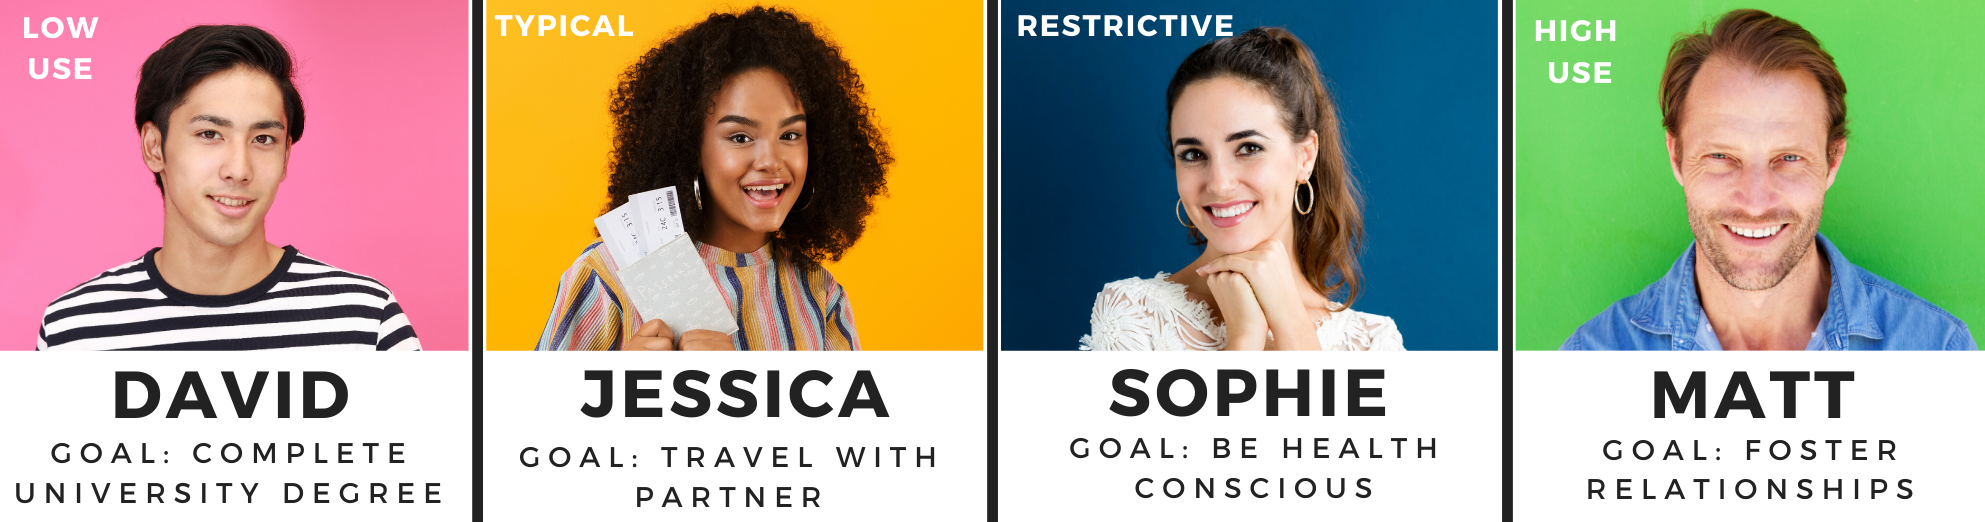
\includegraphics[width=0.9\textwidth, frame]
            {./Med_Fidelity/Med_Report/images/personas_overview.PNG}  
            %{./images/personas_overview.PNG}
        \caption{Personas Overview}
    \end{figure} 
    
    These personas were developed by reviewing the initial research of the application (both desk research and interviews) and the participants of the low fidelity evaluations to refine 'Who is the user?' and 'What is important to the user?' [24]. First need to look at the characteristics identified to describe the behaviour of the users:
        \begin{itemize}
            \item Who? Everyone eats out so personas are all in different age demographics, relationships, employment and income brackets.
            \item What? From the interviews, all 'sometimes' try new places so the personas are mixed. 
            \item When? Users range from eating out at least once per week up to four times per week so each user falls under a different number.
            \item Where? Anywhere, all like options
            \item Why? To share experience with others, so 3/4 of the personas always eat with others.
        \end{itemize}

    Also as identified in the initial research and confirmed by the low fidelity evaluations, there are six factors that are important to the user [24]. Each of these factors are covered by the features of the application. Each persona encompasses three of these factors in their decision process and eating out behaviours.
    \begin{center}
    \begin{tabular}{|l|c|c|c|c|}   
        \hline  
        Factor                                                          & David & Jessica& Sophie   & Matt \\
        \hline \hline
        Matches dietary \textit{(2/12 participants had dietary concerns)}&      &       & Yes       &   \\
        \hline
        Choose by craving \textit{('Taste' is most important factor)}   &       & Yes   &           & Yes \\ 
        \hline
        Word-of-mouth \textit{(91\% based on recommendation)}           &       &       & Yes       & Yes \\ 
        \hline
        Located nearby \textit{(1/3 mentioned as part of decision)}     & Yes   &       &           & Yes \\ 
        \hline
        Menu online \textit{(50\% always, 50\% sometimes look before)}  & Yes   & Yes   & Yes       &  \\
        \hline
        Deal or low cost \textit{(3rd most important factor)}           & Yes   & Yes   &           &  \\
        \hline
        \end{tabular}
    \end{center}
    
 

    \subsubsection{Interaction Scenarios}
    For each of the created persona's a storyboard of their typical interaction with the system was sketched. These scenarios communicate the subsets of user behaviour of the system to assist with ensuring all users needs are met and that the design of the system supports these expectations [33]. Each scenario has 11 slides and uses the template supplied by NNGroup with rough sketches and simple explanations. The scenarios range from unflawed or expected use of \textit{foodie} to challenges and frustrations with existing applications to represent a range of cases. There are four scenarios, all of which can be found in \hyperref[sec:B.2]{Appendix B.2}.
        \begin{enumerate}
            \item David - Student Deals: David wants to eat out with friends but wants to find the cheapest option. He uses Google Maps to look nearby but has to go to each restaurant's website to to view the deals. He struggles to remember all the deals and places he has looked at and the text conversation with his friends is just a mess of links and names. It takes over 20 minutes to find somewhere.
            \item Jessica - Hump Day: Jessica doesn't feel like cooking and so she wants to send some good value options to her partner. She regularly uses the Foodie app and has a list of favourites. She checks which one has a good deal and matches her craving to add to her comparison list. She sends these options to her partner, who in turn remembers somewhere he has been wanting to try and edits the list to send back to her. This place looks great so they decide to go here and Jessica saves it for next time too.
            \item Sophie - Busy Planner: Sophie has a busy day on the road tomorrow so she needs to plan what she is going to have for lunch. This is her least favourite task of planning as she has to look through lots of images of menus on the Zomato app to find what matches her diet. Then she reads through long reviews to get a sense of the place before writing it down in her diary for tomorrow. When tomorrow comes she will decide and have to get directions on Google Maps.
            \item Matt - Lunch at work: Matt is at work and is craving pizza for lunch. He wants to pick somewhere nearby that is preferably recommended by friends. He doesn't like to waste time deciding so he uses the Foodie app since he can filter by pizza and location on the first page and get a quick glance of what his friends think. 
        \end{enumerate}

    \subsubsection{UX Goals}
    When determining the 'success' of the user experience, according to NNGroup, it is important to 'focus on outcomes not the features' [46]. Rather than focus on the service the application is offering, focus on the problem that this application is solving. The problem is that no existing solutions give users what they actually want (the benefits); options to dine out with others based on personal preference (craving, dietary), nearby location and word-of-mouth recommendations.

    These UX Goals were developed by identifying the main user needs, from previous evaluations and research, and then selecting content and functionality requirements to meet them. The goals use SMART principles and together cover all systems requirements [41]. Each goal is a real-world end state that users want to reach [71]. The full details of the UX goals, including their source, measures and link to requirements, can be found in \hyperref[sec:B.3]{Appendix B.3}. 
        \begin{enumerate}
            \item I want to dine out at places that match my dietary requirement.
            \item I want to eat what I am craving.
            \item I want to choose where to eat based on my location. 
            \item I want to view the menu of the restaurant as it relates to me before going there.
            \item I want to learn about the relevant deals of a restaurant.
            \item I want access to the basic information of a restaurant.
            \item I want to compare a variety of restaurants at once.
            \item I want to share the experience of dining out with friends.
            \item I want to dine out at restaurants that have been recommended by word-of-mouth.
            \item I want to re-visit restaurants that I enjoyed.
            \item I want to find new places to eat out.
            \item I want to dine out in my budget.
            \item I want to decide where to dine out in less than 20 minutes.
            \item I want support restaurants without having to leave long reviews.
        \end{enumerate}

% 3.2.2 MEDIUM FIDELITY PROTOTYPE
\subsection{Medium Fidelity Prototype}
Taking into consideration the revised requirements as outlined from the results of the low fidelity prototype evaluations a medium fidelity prototype was created. Figma was chosen due to its browser-based interface, easy-to-use design, prototype functionality and popularity in the UX world [74]. Colour, icons and basic functionality has been implemented. The icons were created using logomkr [75] and any images are sources from the open-source photo collection on canva [73].

    \subsubsection{Interface Design}
    To align with the design principles any metaphors that didn't previously match the material design icons will be updated (Google Maps pin, compass, menu, coupon). Overall the updates ensure user's have clear understanding and awareness that:
        \begin{itemize}
            \item the shareable comparison list is a main feature with clear guidance to get there and understanding of its purpose. $\dashrightarrow$ Change LIST to COMPARE and update 'bookmark' metaphor to 'scales'. For the 'add to compare' icon, enlarge it, add this text and move it to the main area on restaurant page.
            \\ \textit{This will help David with finding options that he can share with his friends instead of having to remember them separately.} 
            \item both the map and menu are filtered by their personal preferences with the ability to expand or minimise these options as needed. $\dashrightarrow$ Add filter bar to MENU page, add shading to selected filters \\ 
            \textit{This will solve Sophie's frustration of wanting to look through multiple menus for her diet without navigating between websites.}
            \item recommendations are by word of mouth, with the option to view all responses as well. $\dashrightarrow$ Add text 'friends' next to recommendations, add option to view all reviews. \\
            \textit{This will save Matt time as he highly values the opinions of friends and wants to make a quick decision.}
            \item they have access to basic information of a restaurant on every relevant page. $\dashrightarrow$ Add overlay with more action icons when select from compare list \\
            \textit{This will assist Jessica with wanting to use her list of saved restaurants as her method of search to send to her partner to view.}
        \end{itemize}        
        
        The below is the interface of the medium fidelity prototype, with any relevant updates outlined. Also note, the application now has a name; foodie. It is simple and fun. It will replace APPNAME in the top navigation bar. 
            \begin{figure} [H]
                \centering
                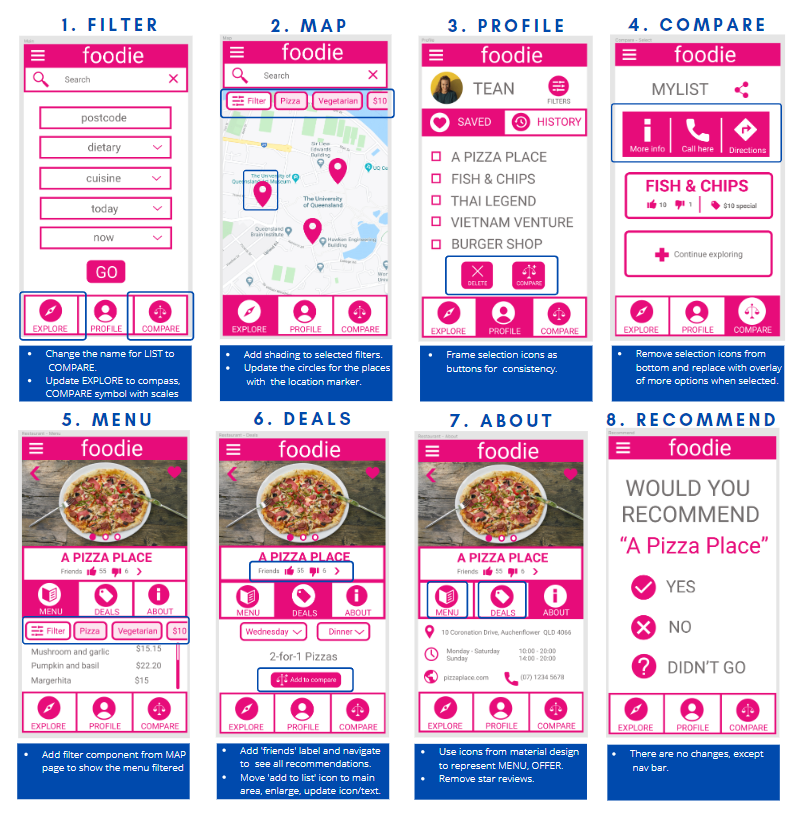
\includegraphics[width=0.9\textwidth, frame]
                    {./Med_Fidelity/Med_Report/images/med_proto_notes.PNG}  
                    %{./images/med_proto_notes.PNG}
                \caption{Medium Prototype - Interface Modifications}
            \end{figure}   
        
        \subsubsection{Interface Functionality}
        Since this is the first digital version of the prototype, the same interaction as the low fidelity prototype was implemented (only one end option for each feature). The functionality at this time mainly includes the navigation between tabs. For the buttons, the 'GO', back arrow and 'continue exploring' navigates to the map, while 'Add to compare' to the compare list. There is also the ability to scroll through the menu once. 
        \begin{figure} [H]
            \centering
            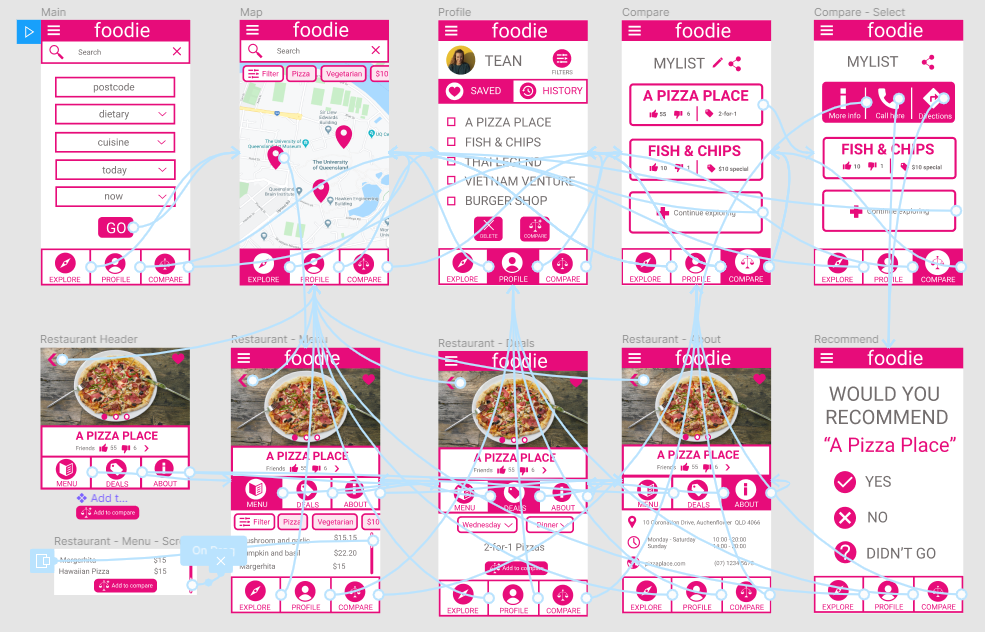
\includegraphics[width=0.9\textwidth, frame]
                {./Med_Fidelity/Med_Report/images/med_proto_func.PNG}  
                %{./images/med_proto_notes.PNG}
            \caption{Medium Prototype - Interface Functionality}
        \end{figure}


% 3.2.3 MEDIUM FIDELITY PROTOTYPE EVALUATION
\subsection{Medium Fidelity Prototype Evaluation}

    \subsubsection{Evaluation Methods}
    Instead of evaluating whether the application assists users with solving a problem the purpose of the evaluations of the medium fidelity is to determine the usability of the application which in turn contributes to shaping the user experience [57]. Any gaps between mental models in the low fidelity prototype have been amended for the medium fidelity prototype and it has been determined that this application is something users want, so now it is a matter of whether they can use it.  

    The think aloud evaluation method requires users to either complete a specific task or walk through all aspects of the application, whilst saying out loud everything they are thinking [42]. This method was chosen as it provides substantial qualitative feedback on the user's experience as it is happening in regards to their expectations of the system. Since the end goal for this application is the same for every user, deciding where to dine out, the process of deciding is different for every user with a wide range of approaches that can be taken with the system.

    The System Usability Scale (SUS) is a set of 10 questions, with both positive and negative responses, that provides a grade for the usability of the system. These questions are a popular staple of evaluation in the user experience industry as they are are cheap and quick process [66]. Since the user is only required to respond with a numerical value, the full picture of why and how users feel about a system may be missing. This is used to supplement the think aloud evaluation as it provides an overall quantitative picture of the user experience after an overload of qualitative feedback [66].
    
    After all evaluations have been completed, the raw data collected from the results of the SUS questionnaire will go through the following steps to effectively analyse the data and get a better understanding of users overall opinion of the systems usability. These steps will provide a SUS Score for each participant, as well as an average, which can be compared against the standard percentile ranks. Also, since the average of results can be skewed by outliers, a distribution of responses is generated which instead shows the median and interquartile range which is not affected by these outliers [35, 26].
        \begin{enumerate}
            \item Convert Raw Data: ODD = Response - 1, EVEN = 5 - Response
            \item Calculate SUS Scores: Total * 2.5 for each participant
            \item  Average for each question: Total / number of participants for each question
            \item Distribution of responses: Boxplot to show distribution of each question
        \end{enumerate}  

    \subsubsection{Evaluation Protocol}
    The purpose of this protocol, structure and consistency, is the same as the low fidelity prototype. The protocol can be viewed in \hyperref[sec:B.4]{Appendix B.4}. Also similarly, users are invited to a Google Form where all instructions, links and surveys are available to them. The form can be viewed in \hyperref[sec:B.5]{Appendix B.5}. After providing consent the user will be directed to an interactive prototype. Each page of the prototype is outlined by a typical android smartphone frame. The slides can be viewed in \hyperref[sec:B.1]{Appendix B.6}. 

    Users are asked to use the app as if they were a first time user interested in the app. They are given no specific task and are asked to speak all thoughts out loud with no interruptions from the evaluator. This is in-line with the Think Aloud evaluation method. In addition to taking note of their use and understanding of components of the prototype, the numerical measures (clicks, errors and time) for the UX goals will also be taken simultaneously. After the user has finished explaining each step of the system as they understand, users will be directed back to the Google Forms to answer the 'Survey Questions' to further measure the UX Goals. Each questions is rated out of 3 (don't agree, neutral, agree). Following these questions, the users will also complete the SUS questionnaire. This is simply the collection of raw data which will be analysed once all evaluations have been completed.
  
    For this evaluation, there are six participants in total. Three of the users will be brand new to the system, whilst the other two took part in the evaluation of the low fidelity prototype. This provides a balance of fresh eyes with no preconceived ideas who can comment on the basic flow of the application, and also those who already have a basic understanding who were able to evaluate if the changes made were appropriate and look at the application in more detail. The raw notes are in \hyperref[sec:B.7]{Appendix B.7}. 


    \subsubsection{Evaluation Results}
    The following provides an overview of the results and feedback from the evaluations and is separated by each persona's ability to complete their scenario. 
        \begin{enumerate}
            \item David - Student Deals
                \begin{itemize}
                    \item Today/now confusing, didn't understand the difference between the two $\dashrightarrow$ 2/5 user's mentioned.
                    \item Wants to be able to filter by price before getting to the map view $\dashrightarrow$ The poorest survey responses were to UX Goal 'I want to dine out in my budget'.
                    \item Liked that there was a dedicated page for deals, though wanted to be able to view this tab first (before menu).
                \end{itemize}

            \item Jessica - Hump Day
                \begin{itemize}
                    \item Went to the saved restaurant but couldn't go to the restaurant information page without adding to the compare list first $\dashrightarrow$ Poor response to 'I could easily access information when needed'
                    \item Tried to find an option to view all deals.
                    \item Wanted to be able to follow partner's saved places instead of just in the list. 
                \end{itemize}

            \item Sophie - Busy Planner
                \begin{itemize}             
                    \item Was able to filter by location, cuisine,  dietary and tomorrow which she felt made the search very custom.
                    \item Wanted to be able to save her preferences for later but couldn't find how to without assistance.
                    \item Still had difficulty finding how to add a restaurant to compare list though was quicker than previously $\dashrightarrow$ Poor responses to both time and survey results for UX Goal 'I want to compare a variety of restaurants at once.'
                    \item After finding places , wasn't sure if compare list was going to be able to save for the next day and wanted to be able to save for future trips. 
                \end{itemize}

            \item Matt - Lunchtime at work
                \begin{itemize}
                    \item Selected to filter by cuisine for the map, but wanted to be able tell which places were popular before having to click into each one
                    \item Once at the restaurant looked at the recommendations and could tell they were friends
                    \item Wanted to be able to go straight here without going to compare list, wanted a 'go here now' option $\dashrightarrow$ Poor response to 'I could easily access information when needed'
                    \item After going to the restaurant wanted to be able to recommend without having to open the app.
                \end{itemize}
        \end{enumerate}

    \subsubsection{Evaluation Analysis}
    The overall interaction of the app was much improved from the low fidelity prototype as users could now progress from the restaurant page to the compare list, and move from compare list to their next desired page (back or forward) without issues. This was confirmed by the positive responses and reduced number of errors to the related UX measures. The first step in understanding the data was to complete the data analysis steps of the raw data collected from the SUS questionnaire to calculate the scores and view the distribution. The data and graphs associated with the analysis of this raw data can be viewed in \hyperref[sec:B.8]{Appendix B.8}.

    In terms of usability, as per the SUS analysis the grading of the system overall was a low A with an above average score in the 82nd percentile. However, the scoring was as low as 62.5\% (C - below average) to 95\% (A - above average). 
    \begin{figure}[H]
        \centering
        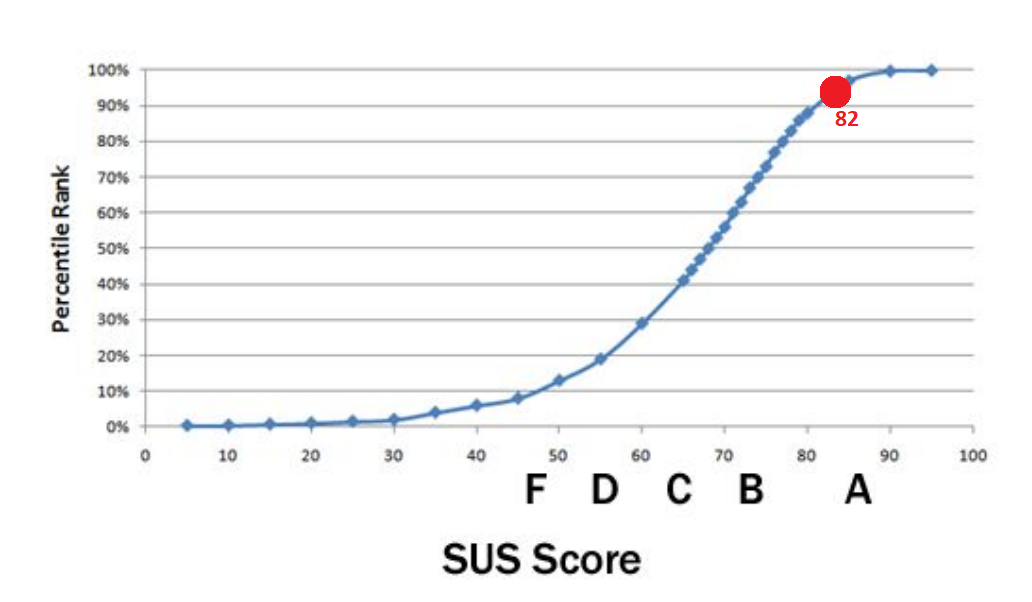
\includegraphics[width=0.5\textwidth, frame]
            {./Med_Fidelity/Med_Report/images/Med_SUS_Grade.PNG} 
        \caption{SUS Grade}
    \end{figure}   
        
   The lowest scoring questions was 'I thought there was too much inconsistency in this system' with an average of 2.8. The highest scoring question was (reverse) 'I think that I would need the support of a technical person to be able to use this system' with 3.66, closely followed with 'I found the system unnecessarily complex' with 3.5. All other questions were either rated overall 3.16 or 3.33. This suggests that the system is easy to use in terms of technical complexity, however there is still too much thought process involved with moving through the system.
   
   The think aloud evaluations identified that the main issue contributing to this inconsistency in this iteration was the availability of options for different actions. This also aligned with three UX goals not being met. The first UX goal not achieved is 'I want to dine out in my budget' which had to poorest response to survey questions. Users want to be able to filter by budget on the first page, and agreed the now option is redundant. The second UX goal is 'I want to compare a variety of restaurants at once', which caused the highest number of errors when moving from restaurant to compare. Users want a broader view of the places on the map view with differentiation of restaurants based on popularity before selecting an irrelevant restaurant (different colour or icons with legends). Also, although the time from restaurant page to compare list was greatly reduced, many of the users still had difficult finding the 'add to compare' button as it was often hidden. 

    The third UX goal that users was 'I could easily access information when needed' which was only met sometimes. Users want the ability to be assisted with going to a restaurant straight from the restaurant page without proceeding to the compare screen (more buttons). On the restaurant page no-one used the bottom tab and so instead this will be replaced by the popular action buttons. Additionally, users wanted to be able to access more information on the places recorded in their profile without having to add them to the compare list first. Most users commented they usually wouldn't select more than one restaurant at a time, so instead of checkboxes the same overlay as the compare page will be used (more info, add to compare and delete as the options).


    \end{document}